% Options for packages loaded elsewhere
\PassOptionsToPackage{unicode}{hyperref}
\PassOptionsToPackage{hyphens}{url}
\documentclass[
  american,
  11pt,
]{article}
\usepackage{xcolor}
\usepackage[margin=25mm]{geometry}
\usepackage{amsmath,amssymb}
\setcounter{secnumdepth}{-\maxdimen} % remove section numbering
\usepackage{iftex}
\ifPDFTeX
  \usepackage[T1]{fontenc}
  \usepackage[utf8]{inputenc}
  \usepackage{textcomp} % provide euro and other symbols
\else % if luatex or xetex
  \usepackage{unicode-math} % this also loads fontspec
  \defaultfontfeatures{Scale=MatchLowercase}
  \defaultfontfeatures[\rmfamily]{Ligatures=TeX,Scale=1}
\fi
\usepackage{lmodern}
\ifPDFTeX\else
  % xetex/luatex font selection
\fi
% Use upquote if available, for straight quotes in verbatim environments
\IfFileExists{upquote.sty}{\usepackage{upquote}}{}
\IfFileExists{microtype.sty}{% use microtype if available
  \usepackage[]{microtype}
  \UseMicrotypeSet[protrusion]{basicmath} % disable protrusion for tt fonts
}{}
\makeatletter
\@ifundefined{KOMAClassName}{% if non-KOMA class
  \IfFileExists{parskip.sty}{%
    \usepackage{parskip}
  }{% else
    \setlength{\parindent}{0pt}
    \setlength{\parskip}{6pt plus 2pt minus 1pt}}
}{% if KOMA class
  \KOMAoptions{parskip=half}}
\makeatother
\usepackage{longtable,booktabs,array}
\newcounter{none} % for unnumbered tables
\usepackage{calc} % for calculating minipage widths
% Correct order of tables after \paragraph or \subparagraph
\usepackage{etoolbox}
\makeatletter
\patchcmd\longtable{\par}{\if@noskipsec\mbox{}\fi\par}{}{}
\makeatother
% Allow footnotes in longtable head/foot
\IfFileExists{footnotehyper.sty}{\usepackage{footnotehyper}}{\usepackage{footnote}}
\makesavenoteenv{longtable}
\usepackage{graphicx}
\makeatletter
\newsavebox\pandoc@box
\newcommand*\pandocbounded[1]{% scales image to fit in text height/width
  \sbox\pandoc@box{#1}%
  \Gscale@div\@tempa{\textheight}{\dimexpr\ht\pandoc@box+\dp\pandoc@box\relax}%
  \Gscale@div\@tempb{\linewidth}{\wd\pandoc@box}%
  \ifdim\@tempb\p@<\@tempa\p@\let\@tempa\@tempb\fi% select the smaller of both
  \ifdim\@tempa\p@<\p@\scalebox{\@tempa}{\usebox\pandoc@box}%
  \else\usebox{\pandoc@box}%
  \fi%
}
% Set default figure placement to htbp
\def\fps@figure{htbp}
\makeatother
% definitions for citeproc citations
\NewDocumentCommand\citeproctext{}{}
\NewDocumentCommand\citeproc{mm}{%
  \begingroup\def\citeproctext{#2}\cite{#1}\endgroup}
\makeatletter
 % allow citations to break across lines
 \let\@cite@ofmt\@firstofone
 % avoid brackets around text for \cite:
 \def\@biblabel#1{}
 \def\@cite#1#2{{#1\if@tempswa , #2\fi}}
\makeatother
\newlength{\cslhangindent}
\setlength{\cslhangindent}{1.5em}
\newlength{\csllabelwidth}
\setlength{\csllabelwidth}{3em}
\newenvironment{CSLReferences}[2] % #1 hanging-indent, #2 entry-spacing
 {\begin{list}{}{%
  \setlength{\itemindent}{0pt}
  \setlength{\leftmargin}{0pt}
  \setlength{\parsep}{0pt}
  % turn on hanging indent if param 1 is 1
  \ifodd #1
   \setlength{\leftmargin}{\cslhangindent}
   \setlength{\itemindent}{-1\cslhangindent}
  \fi
  % set entry spacing
  \setlength{\itemsep}{#2\baselineskip}}}
 {\end{list}}
\usepackage{calc}
\newcommand{\CSLBlock}[1]{\hfill\break\parbox[t]{\linewidth}{\strut\ignorespaces#1\strut}}
\newcommand{\CSLLeftMargin}[1]{\parbox[t]{\csllabelwidth}{\strut#1\strut}}
\newcommand{\CSLRightInline}[1]{\parbox[t]{\linewidth - \csllabelwidth}{\strut#1\strut}}
\newcommand{\CSLIndent}[1]{\hspace{\cslhangindent}#1}
\ifLuaTeX
\usepackage[bidi=basic,shorthands=off]{babel}
\else
\usepackage[bidi=default,shorthands=off]{babel}
\fi
\ifLuaTeX
  \usepackage{selnolig} % disable illegal ligatures
\fi
\setlength{\emergencystretch}{3em} % prevent overfull lines
\providecommand{\tightlist}{%
  \setlength{\itemsep}{0pt}\setlength{\parskip}{0pt}}
\usepackage{bookmark}
\IfFileExists{xurl.sty}{\usepackage{xurl}}{} % add URL line breaks if available
\urlstyle{same}
\hypersetup{
  pdftitle={Efficient weak-form estimation under correlated measurement error: fixed-horizon information limits and the cost of boundary-free test functions},
  pdflang={en-US},
  hidelinks,
  pdfcreator={LaTeX via pandoc}}

\title{Efficient weak-form estimation under correlated measurement
error: fixed-horizon information limits and the cost of boundary-free
test functions}
\author{}
\date{}

\begin{document}
\maketitle

\subsection{Abstract}\label{abstract}

Weak-form dynamical identification avoids differentiating noisy
measurements, but removing boundary terms also discards information. For
deterministic ODEs observed in stationary Ornstein-Uhlenbeck measurement
error, we characterize the closure of boundary-free adjoint influences:
it is exactly the covariance-dual subspace orthogonal to initial-state
sensitivities. This gives a sharp local covariance bound equal to the
inverse initial-state Schur complement, even when the initial state is
known. We construct its optimal influence and an explicit generalized
test function with endpoint jumps. Compact tests attain the bound as an
infimum. Correct-covariance weak generalized least squares approaches
this bound for dense test spans, in a sequential small-noise limit with
controlled quadrature and regular pilots. A finite Hermite expansion
supplies exact coupled polynomial residual weights. A fixed-horizon
two-point bound separates this efficiency question from consistency
under denser sampling. Experiments test a smoothed scalar optimal
function with a fitted pilot and nested 30-, 120- and 480-window Van der
Pol families, comparing physical OU and iid weights. The scalar
fitted-pilot median error decreases from 0.224 to 0.060. Van der Pol
empirical RMSE at 0.5\% noise is 0.00174, versus the weak reference
0.00169; the 5\% experiment retains excess error. Bias and dispersion
are reported separately. The contribution identifies which information
weak equations can retain and how covariance weighting and test-space
approximation govern its recovery.

\textbf{Keywords:} weak-form identification; correlated measurement
error; fixed-domain asymptotics; Fisher information; polynomial
covariance; errors in variables.

\subsection{1. Introduction}\label{introduction}

Data acquisition for dynamical identification involves three choices:
how often to sample, how long to observe, and how many independent
recordings to acquire. These choices have different statistical effects.
Sampling more frequently improves numerical integration while repeatedly
observing the same correlated error path. A longer recording may
encounter new noise but little additional parameter sensitivity.
Independent recordings can add information even when each individual
trajectory remains statistically unresolved.

Sparse identification of nonlinear dynamics represents a vector field
through a library and selects active coefficients {[}1{]}. Integral
formulations reduce sensitivity to numerical differentiation {[}2{]},
and weak formulations transfer differentiation to test functions {[}3,
4{]}. Their regression matrices still contain noisy states. Numerical
resolution, feature bias, residual covariance and model selection
interact, so reducing quadrature error does not by itself establish
statistical consistency.

The distinction between fixed-domain and increasing-domain observations
is classical in Gaussian process inference {[}5{]}. Ying established
fixed-domain results for exponential covariance parameters {[}6{]}, and
Zhang used equivalence of Gaussian measures to explain inconsistent
covariance estimation in the Matérn family {[}7{]}. Those results
concern covariance parameters. Here the covariance is common across
parameters, and the parameter enters the deterministic mean through an
ODE. The same measure-equivalence mechanism supplies an
estimator-independent limit, with an explicit norm determined by
dynamical sensitivities.

Continuous-time regression with correlated errors has an established
optimal-design theory, including optimal signed measures with endpoint
masses. Dette, Pepelyshev and Zhigljavsky derive continuous-record best
linear unbiased estimators and efficient discrete designs for triangular
covariance kernels {[}8{]}. Dynamical sensitivities define a local
regression in this framework. Finite limiting precision and endpoint
information are therefore precedents for our weak-estimation analysis.

The continuum-data theory of WSINDy studies uncorrelated measurement
errors and library-dependent consistency {[}9{]}. Fixed physical
correlation time defines a different experiment: adjacent correlations
approach one as the mesh is refined. Correlation induced by filtering
independently sampled errors also requires distinguishing a physical
filter scale from a fixed number of sample indices. Our analysis
concerns a fixed covariance process observed at increasingly dense
times.

Our main result identifies the complete boundary-free adjoint influence
class and constructs the influence attaining its sharp information
reference in covariance-norm closure. Correct temporal covariance and
dense test spans then yield a conditional, sequential small-noise
efficiency result for WENDy-like estimation. An explicit OU adjoint
construction and exact polynomial residual weights make the reference
computable. Continuous-regression BLUE, Gaussian projection and Hermite
identities are established results {[}8, 10{]}; the contribution is
their precise connection through the ODE adjoint range, including the
boundary restriction and the order of limits. Two experiments test the
resulting predictions.

\subsection{2. Related estimation
methods}\label{related-estimation-methods}

WENDy treats weak parameter estimation as an errors-in-variables problem
and iteratively updates a linearized residual covariance {[}11{]}. It
retains perturbations of both the feature matrix and the response. We
use the same coupled residual and compute every Gaussian order for
polynomial features under the specified OU model. First-order truncation
recovers the structure motivating weak reweighting, with temporal
covariance inserted explicitly. Residual covariance is distinct from the
covariance of the nonlinear coefficient estimator.

Errors-in-variables effects have a substantial statistical literature
{[}12{]}. Gaussian correction of nonlinear functions of a noisy mean
also precedes weak identification {[}13{]}. Hermite correction removes
pointwise polynomial bias when marginal noise variance is known; it does
not remove random design--response coupling. Generalized smoothing and
profiling estimate ODE parameters through a different compromise between
model fidelity and observation error {[}14{]}. The information bound
applies to these alternatives when they observe the same path
experiment.

WmSINDy combines weak regression with simultaneous dynamics and noise
reconstruction {[}15{]}. We distinguish the large fixed-window
regression-component study from a separate paired execution of the
complete adaptive author WSINDy, WENDy and WmSINDy pipelines. The latter
retains noise estimation or reconstruction and adaptive test-function
selection; WENDy supplies structure for parameter estimation.
Ensemble-SINDy uses bootstrap aggregation to quantify feature inclusion
{[}16{]}. Resampling one recorded path and acquiring independent
physical recordings are different operations: the latter changes the
number of independent path experiments in the information calculation.

\subsection{3. Observation model and weak
equations}\label{observation-model-and-weak-equations}

Let \(x_\theta:[0,T]\to\mathbb R^d\) be a deterministic ODE trajectory.
In the polynomial setting,

\[
x'_i=f_i(x)=\sum_{j=1}^{p}\xi^*_{ji}\vartheta_j(x),\qquad i=1,\ldots,d.
\]

The library contains all true terms. Observations are
\(Y(t)=x_\theta(t)+\varepsilon(t)\), with independent stationary OU
coordinates {[}17{]} and common-across-parameter covariance

\[
C_j(s,t)=\sigma_j^2\exp(-|s-t|/\tau_j),\qquad \sigma_j>0,\quad\tau_j>0.
\]

The continuous record is a statistical reference experiment; actual data
are evaluations \(y_n=Y(t_n)\) at mesh \(h\). Initial conditions are
known unless stated otherwise; unknown initial conditions would
introduce nuisance sensitivities.

Fix \(K\) test functions \(\phi_k\in C_c^2(0,T)\). Their positions and
full support widths \(L\) remain fixed as \(h\) decreases. Let
\(\mathcal Q_h\) be composite trapezoidal quadrature with weights
\(w_n\). Clean weak quantities are

\[
G^0_{kj}=\int_0^T\phi_k\vartheta_j(x)\,dt,\qquad
b^0_{ki}=-\int_0^T\phi'_kx_i\,dt,\qquad b^0=G^0\xi^*.
\]

Noisy matrices use corrected polynomial features
\(\widetilde\vartheta_j\), defined in Section 5:

\[
(G_h)_{kj}=\mathcal Q_h(\phi_k\widetilde\vartheta_j(y)),\qquad
(b_h)_{ki}=-\mathcal Q_h(\phi'_ky_i).
\]

Physical OU infill sets \(\rho(h)=\exp(-h/\tau)\) with fixed \(T,\tau\).
An iid discrete control has independent error of fixed per-sample
variance. Fixed-index AR(1) instead keeps \(\rho<1\) constant, making
the physical correlation time \(-h/\log\rho\to0\). These models have
different continuum limits.

\subsection{4. An estimator-independent fixed-horizon
limit}\label{an-estimator-independent-fixed-horizon-limit}

\subsubsection{4.1. OU translation
geometry}\label{ou-translation-geometry}

The stationary OU process satisfies
\(d\varepsilon_j=-\varepsilon_jdt/\tau_j+\sqrt{2\sigma_j^2/\tau_j}\,dW_j\),
with an independent initial value
\(\varepsilon_j(0)\sim N(0,\sigma_j^2)\). Its Cameron--Martin space is
\(H^1([0,T];\mathbb R^d)\) as a set, with norm

\[
\|g\|_{\mathcal H}^2=\sum_j\left\{\frac{g_j(0)^2}{\sigma_j^2}+
\frac{\tau_j}{2\sigma_j^2}\int_0^T(g'_j+g_j/\tau_j)^2\,dt\right\}.
\]

Transforming a path into its initial value and innovation path
\(z(t)-z(0)+\tau_j^{-1}\int_0^tz(s)ds\) separates the normal initial
observation from scaled Brownian motion. Translation by \(g\) gives an
initial shift and Brownian drift \(g'+g/\tau_j\). The classical
translation theorem {[}18{]} gives the norm. Equivalently,

\[
\|g\|_{\mathcal H}^2=\sum_j\left\{\frac{\tau_j}{2\sigma_j^2}\int_0^T(g'_j)^2dt+
\frac1{2\sigma_j^2\tau_j}\int_0^Tg_j^2dt+
\frac{g_j(0)^2+g_j(T)^2}{2\sigma_j^2}\right\}.
\]

The endpoint terms encode stationary initial noise. Zero initial error
would define a different experiment.

\textbf{Theorem 1 (fixed-horizon two-point bound).} Suppose
\(x_\theta\in H^1\) and all parameters share the stated positive OU
covariance. For distinct \(\theta,\eta\), put \(\delta=\|\theta-\eta\|\)
and \(d_{\theta\eta}=\|x_\theta-x_\eta\|_{\mathcal H}\). Every estimator
from any finite grid satisfies

\[
\max_{v\in\{\theta,\eta\}}P_v\{\|\widehat\theta_h-v\|\geq\delta/2\}
\geq\Phi(-d_{\theta\eta}/2)>0.
\]

No denser-grid estimator sequence is consistent in probability at every
parameter of a nontrivial family. Moreover,

\[
\max_{v\in\{\theta,\eta\}}E_v\|\widehat\theta_h-v\|^2
\geq\frac{\delta^2}{4}\Phi(-d_{\theta\eta}/2).
\]

\textbf{Proof.} The mean difference belongs to the common
Cameron--Martin space, making the path laws equivalent; this is the
common-covariance case of Gaussian measure equivalence {[}19{]}. Under
the first law the log likelihood ratio of the second is normal with mean
\(-d_{\theta\eta}^2/2\) and variance \(d_{\theta\eta}^2\). Their total
variation is \(2\Phi(d_{\theta\eta}/2)-1\). Sampling cannot increase
total variation. A nearest-parameter test derived from an estimator can
err only if that estimator is at least \(\delta/2\) from the generating
parameter. The sum of testing errors is at least one minus total
variation, giving the probability bound. Multiplying the estimation
probability by \(\delta^2/4\) gives the risk bound. Both bounds hold at
every mesh. \(\square\)

A constant estimator can be consistent at one parameter. The theorem
excludes consistency throughout the family. The equivalence-based
obstruction is established fixed-domain theory {[}7{]}; its norm and
quantitative specialization here concern ODE mean trajectories. The
bound includes adaptive weak functions and full-path inference.

\subsubsection{4.2. Continuous-record information and scalar weak
ratios}\label{continuous-record-information-and-scalar-weak-ratios}

\textbf{Proposition 1 (continuous-record information).} If
\(\theta\mapsto x_\theta\) is differentiable in \(\mathcal H\) and
\(s_r=\partial_{\theta_r}x_\theta\), continuous-record Fisher
information is

\[
\mathcal I_{rs}(\theta)=\langle s_r,s_s\rangle_{\mathcal H}.
\]

The Gaussian mean-score identity proves the assertion: the directional
score has variance equal to the squared Cameron-Martin norm of its
sensitivity. Its inverse is the Cramér--Rao covariance bound for regular
unbiased estimators, when nonsingular. Biased estimators require the
corresponding bias derivative; finite-horizon maximum likelihood need
not attain the unbiased bound.

For \(x_a(t)=x_0e^{at}\) with known \(x_0\), \(s(t)=x_0te^{at}\) and

\[
\mathcal I_T(a)=\frac{\tau x_0^2}{2\sigma^2}
\int_0^Te^{2at}[1+(a+\tau^{-1})t]^2\,dt.
\]

On a uniform grid, exact innovations give

\[
\mathcal I_h(a)=\frac{s(0)^2}{\sigma^2}+
\frac{\sum_{n=1}^N[s(t_n)-\rho s(t_{n-1})]^2}{\sigma^2(1-\rho^2)}
\longrightarrow\mathcal I_T(a),\qquad\rho=e^{-h/\tau}.
\]

Nested grids give increasing information bounded by \(\mathcal I_T\).
The limit follows from a Riemann sum of squared sensitivity innovations.
Statistical saturation therefore concerns the full experiment.

For \(D_\phi=\int\phi x_a\ne0\), a scalar weak ratio has limit

\[
\widehat a_h=\frac{-\mathcal Q_h(\phi'Y)}{\mathcal Q_h(\phi Y)}
\longrightarrow a+\frac{A}{D_\phi+B},\qquad
A=\int(-\phi'-a\phi)\varepsilon,\quad B=\int\phi\varepsilon.
\]

OU path continuity gives almost sure convergence of the quadratures. The
weights \(\phi\) and \(-\phi'-a\phi\) are independent: dependence would
make a nonzero compactly supported function solve a homogeneous
first-order equation. The OU kernel is strictly positive on nonzero
weights, so \((A,B)\) is nondegenerate Gaussian. Positive conditional
variance of \(A\) given \(B\) and positive denominator density at zero
imply infinite absolute and squared error moments of the unguarded
ratio. Its empirical summaries should use quantiles or explicit guards.

The influence \(\ell=(-\phi'-a\phi)/D_\phi\) has Gaussian variance
\(V_\phi=\iint\ell(u)C(u,v)\ell(v)dudv\). Differentiating the weak
identity gives \(\int\ell s=1\). Cauchy--Schwarz in the covariance RKHS
gives

\[
1\leq V_\phi\mathcal I_T(a),\qquad
\operatorname{Eff}_\phi=[\mathcal I_T(a)V_\phi]^{-1}\leq1.
\]

This efficiency concerns the Gaussian linearization; it is not the
unguarded ratio's variance.

\subsubsection{4.3. Exact boundary-free influence
class}\label{exact-boundary-free-influence-class}

Let \(J\in C^1([0,T];\mathbb R^{d\times d})\), and let the invertible
fundamental matrix satisfy \(Z'=JZ\), \(Z(0)=I_d\). Put \(A h=h'-Jh\)
and \(A^*\phi=-\phi'-J^T\phi\). Sensor coordinates have independent
stationary OU covariance with fixed positive scales. Its Cameron--Martin
space \(\mathcal H\) is \(H^1\) with the OU inner product. Write
\(\mathcal E=\mathcal H'\) for its continuous dual, equipped with the
covariance norm

\[
\|\lambda\|_C^2=\langle\lambda,C\lambda\rangle,
\qquad
\langle C^{-1}g,h\rangle=\langle g,h\rangle_{\mathcal H}.
\]

This definition includes ordinary integrated influences and endpoint
evaluation measures. It is the variance norm of the associated Gaussian
linear observation; the noise path itself need not belong to
\(\mathcal H\).

\textbf{Proposition 2 (exact range and closure).} In \(L^2\),

\[
A^*H_0^1
=\left\{\ell\in L^2:\int_0^T Z(t)^T\ell(t)dt=0\right\}.
\]

The range of compactly supported smooth tests is dense in this space in
\(L^2\). Its closure in \(\mathcal E\) is exactly

\[
\mathcal M=\overline{A^*C_c^\infty}^{\|\cdot\|_C}
=\{\lambda\in\mathcal E:\langle\lambda,Z_j\rangle=0, j=1,\ldots,d\}.
\]

Consequently \(\mathcal M\) has codimension \(d\).

\textbf{Proof.} Since \(Z^TA^*\phi=-(Z^T\phi)'\), zero endpoint values
imply the moment constraint. Conversely, for an \(L^2\) influence with
zero moment,

\[
\phi(t)=-Z(t)^{-T}\int_0^t Z(s)^T\ell(s)ds
\]

belongs to \(H_0^1\) and satisfies \(A^*\phi=\ell\). Approximation in
\(H_0^1\) by \(C_c^\infty\) and continuity of \(A^*:H_0^1\to L^2\) give
\(L^2\) density. For the stronger closure statement, a function
\(h\in\mathcal H\) annihilates every \(A^*\phi\) if and only if \(Ah=0\)
distributionally, hence \(h=Zc\). The Hahn--Banach annihilator
characterization of a closed subspace then gives the stated closure in
\(\mathcal H'\). The columns of \(Z\) are linearly independent elements
of \(\mathcal H\), so their dual constraints have rank \(d\).
\(\square\)

Zero values at the endpoints do not imply compact support. Equality for
literal compact tests, without a closure or an \(H_0^1\) qualification,
would be false. The relevant closure uses the covariance norm, which is
equivalent to the dual Sobolev norm for this positive OU model.

\subsubsection{4.4. Sharp information and optimal
influence}\label{sharp-information-and-optimal-influence}

Let \(S=[S_1,\ldots,S_p]\in\mathcal H^p\) be coefficient sensitivities,
and form the joint information blocks for \(S\) and \(Z\). Assume
\(\mathcal I_{uu}\) and the Schur complement are positive definite. Set

\[
R=S-Z\mathcal I_{uu}^{-1}\mathcal I_{u\theta},
\qquad
\mathcal I_e=\mathcal I_{\theta\theta}
-\mathcal I_{\theta u}\mathcal I_{uu}^{-1}\mathcal I_{u\theta}.
\]

Projection and best linear unbiased estimation in correlated continuous
regression are classical {[}8{]}. Here the adjoint-range
characterization identifies exactly which dynamical weak influences obey
that projection.

\textbf{Theorem 2 (sharp boundary-free influence covariance).} Let
\(\Lambda=[\lambda_1,\ldots,\lambda_p]\in\mathcal M^p\) satisfy
\(\langle\lambda_r,S_s\rangle=\delta_{rs}\). Its Gaussian influence
covariance obeys

\[
V(\Lambda)\succeq\mathcal I_e^{-1}.
\]

The bound is attained in \(\mathcal M\) by the matrix-valued dual
influence

\[
\Lambda_*=C^{-1}R\,\mathcal I_e^{-1}.
\]

It is the infimum for normalized compact-test influences. It is a
minimum among literal compact tests only when \(\Lambda_*\) belongs to
their adjoint range.

\textbf{Proof.} The \(\mathcal H\) projection makes
\(\langle C^{-1}R,Z\rangle=0\) and
\(\langle C^{-1}R,S\rangle=\mathcal I_e\). Thus \(\Lambda_*\) meets both
constraints and has covariance \(\mathcal I_e^{-1}\). The difference
\(\Delta=\Lambda-\Lambda_*\) pairs to zero with both \(S\) and \(Z\),
hence with \(R\). Covariance cross terms vanish and

\[
V(\Lambda)=\mathcal I_e^{-1}+V(\Delta).
\]

For attainability as an infimum, approximate each column of
\(\Lambda_*\) by compact-test influences in covariance norm. Their
normalization matrices converge to \(I_p\) by continuous pairing with
\(S\); right-multiplication by their inverse transpose enforces exact
normalization while preserving the range and covariance convergence.
\(\square\)

This is a matrix statement. Dividing a vector influence by a scalar
information is valid only when \(p=1\). The information loss is exactly
\(\mathcal I_{\theta u}\mathcal I_{uu}^{-1}\mathcal I_{u\theta}\);
covariance inflation is
\(\mathcal I_e^{-1}-\mathcal I_{\theta\theta}^{-1}\). There is no
direction-independent scalar loss percentage in general.

\subsubsection{4.5. Explicit optimal OU
test}\label{explicit-optimal-ou-test}

For a scalar coordinate with \(g\in H^2\), integration by parts in the
stationary OU norm gives the dual measure

\[
C^{-1}g=
\frac{g-\tau^2g''}{2\sigma^2\tau}\,dt
+\frac{g(0)-\tau g'(0)}{2\sigma^2}\delta_0
+\frac{g(T)+\tau g'(T)}{2\sigma^2}\delta_T.
\]

For independent coordinates the formula applies coordinatewise, using
their respective scales. If only \(g\in H^1\), the Riesz representative
remains well-defined in \(\mathcal H'\) but need not be a density plus
finite endpoint measures.

For a smooth optimal representative write
\(\Lambda_*=m(t)dt+m_0\delta_0+m_T\delta_T\). On the open interval an
adjoint test matrix is

\[
\Phi_*(t)=-Z(t)^{-T}
\left[Z(0)^Tm_0+\int_0^t Z(s)^Tm(s)ds\right].
\]

Extend it by zero outside the observation interval. Its endpoint jumps
supply \(m_0=-\Phi_*(0+)\) and \(m_T=\Phi_*(T-)\), and distributionally
\(A^*\Phi_*=\Lambda_*\). These formulas include the initial atom;
omitting it in the cumulative integral is incorrect. The annihilation
condition supplies the terminal jump. Cutoff and smoothing approximate
this generalized test in covariance norm. These measures describe a
statistical reference; the implemented estimators keep compact tests and
add no explicit boundary observation terms.

For scalar exponential dynamics, \(z=e^{at}\), \(s=x_0te^{at}\),
\(k=\mathcal I_{au}/\mathcal I_{uu}\) and \(g=e^{at}(x_0t-k)\). Define

\[
A_0=\frac{(1-\tau^2a^2)x_0}{2\sigma^2\tau},\qquad
B_0=\frac{-(1-\tau^2a^2)k-2\tau^2ax_0}{2\sigma^2\tau},
\]

\[
q_0=\frac{-k-\tau(x_0-ak)}{2\sigma^2},\qquad
F_j(t)=\int_0^t s^je^{2as}ds.
\]

Then

\[
\phi_*(t)=-\frac{e^{-at}}{\mathcal I_e}
[q_0+A_0F_1(t)+B_0F_0(t)].
\]

For \(a\ne0\), \(F_0=\operatorname{expm1}(2at)/(2a)\) and
\(F_1=[e^{2at}(2at-1)+1]/(4a^2)\); their continuous limits at \(a=0\)
are \(t\) and \(t^2/2\). A pilot coefficient substitutes into this
expression before a compact cutoff is applied. The explicit multivariate
fundamental-matrix expression is an analytical identity, not a guarantee
of stable numerical inversion of \(Z(t)\); strongly contracting dynamics
can make that inversion ill-conditioned.

\subsubsection{4.6. Correct-covariance GLS and dense
spans}\label{correct-covariance-gls-and-dense-spans}

For tests \(\phi_k\), put \(\lambda_k=A^*\phi_k\),
\(D_{kr}=\langle\lambda_k,S_r\rangle\) and
\(\Sigma_{k\ell}=\langle\lambda_k,C\lambda_\ell\rangle\). Remove exact
linear dependencies. If \(D\) has full column rank, covariance-weighted
weak regression has local influence and covariance

\[
P=(D^T\Sigma^{-1}D)^{-1}D^T\Sigma^{-1},\qquad
V_K=(D^T\Sigma^{-1}D)^{-1}.
\]

WENDy's covariance iteration motivates this construction {[}11{]}, but
the released iid covariance is not the correct physical-OU covariance.
Under polynomial features Proposition 3 supplies the complete coupled
residual weights. Its order-one term determines the small-noise
efficient influence; higher orders correct residual uncertainty at
finite amplitude without by themselves removing coefficient-estimator
bias.

\textbf{Corollary 1 (small-noise, dense-span efficiency).} Let the noise
be \(\epsilon Z_C\) with known covariance shape \(C\). Assume a smooth
identifiable parameterization, a generating parameter interior to a
compact parameter set, consistent pilots, consistent covariance-shape
weights and quadrature error \(o(\epsilon)\). For each fixed finite test
family assume a regular local weak solution with the GLS linearization.
For the covariance conclusion additionally assume uniform integrability
of \(\|\epsilon^{-1}(\widehat\theta_{K,\epsilon}-\theta)\|^2\). A
sufficient implementation uses a uniformly stable smooth local solve,
Gaussian moment control on the local Taylor remainder, and bounded
fallback outside the regular region whose probability is
\(o(\epsilon^2)\). Then

\[
\epsilon^{-1}(\widehat\theta_{K,\epsilon}-\theta)
\Rightarrow N(0,V_K),\qquad
\epsilon^{-2}\operatorname{Cov}(\widehat\theta_{K,\epsilon})\to V_K.
\]

If nested test-influence spans are dense in \(\mathcal M\), then

\[
V_K\longrightarrow\mathcal I_{e,C}^{-1}.
\]

\textbf{Proof.} For fixed \(K\), a first-order expansion of the weak
equations gives \(D(\widehat\theta-\theta)=\epsilon r_1+o_p(\epsilon)\)
with the GLS map above. Consistent pilots and weights change the leading
map by \(o_p(1)\); derivatives of pilot-dependent tests multiply the
zero clean residual. Gaussianity gives the distributional assertion; the
stated risk condition justifies covariance convergence. In the Gaussian
dual space, finite-family information is the Gram matrix of the
orthogonal projection of \(C^{-1}R\) onto its test span. Density gives
projection convergence, and nested spans give increasing information;
continuity of inversion at positive definite \(\mathcal I_e\) gives
covariance convergence. \(\square\)

The conclusion is sequential: first small noise and controlled
quadrature for fixed \(K\), then dense spans. A diagonal joint limit
requires uniform remainder, conditioning and covariance-weight control
that are not supplied here. This theorem concerns regular WENDy-like
weak estimation with correct covariance and supplied identifiable
structure, not all implementations called WENDy, finite-noise sparse
selection, or a universal plateau for misspecified iid weighting. A
fixed basis cutoff must be compatible with the density assumption;
discarding an informative direction permanently can invalidate it.

\subsection{5. Exact polynomial weak-residual
covariance}\label{exact-polynomial-weak-residual-covariance}

\subsubsection{5.1. Finite Hermite
expansion}\label{finite-hermite-expansion}

Assume a common \(\tau\) for independent coordinates, and set
\(v_j=\sigma_j^2\). Define \(H_0=1\), \(H_1=u\),
\(H_{q+1}=uH_q-qvH_{q-1}\) and corrected monomials
\(\widetilde\vartheta_\beta(y)=\prod_jH_{\beta_j}(y_j;v_j)\). Their
expectation given \(x\) is \(x^\beta\). This Gaussian debiasing
construction {[}13{]} centers the polynomial residual at the true
coefficients.

For continuum residual \(r_{ki}=b_{ki}-(G\xi^*)_{ki}\), polynomial
expansion gives

\[
r_{ki}=\sum_{1\leq|\alpha|\leq p_*}\int_0^Tc_{ki,\alpha}(t)H_\alpha(\varepsilon(t);v)dt,
\]

where \(p_*\geq1\) is the relevant maximum degree,
\(H_\alpha=\prod_jH_{\alpha_j}\) and

\[
c_{ki,\alpha}=-\mathbf1_{\{\alpha=e_i\}}\phi'_k
-\phi_k\frac{\partial^\alpha f_i(x)}{\alpha!}.
\]

The response and feature perturbations share this coefficient and retain
their cross-covariance.

\textbf{Proposition 3 (exact covariance).} Under these assumptions,

\[
\operatorname{Cov}(r_{ki},r_{\ell m})=
\sum_{1\leq|\alpha|\leq p_*}\alpha!\prod_jv_j^{\alpha_j}
\int_0^T\int_0^Tc_{ki,\alpha}(s)c_{\ell m,\alpha}(t)
e^{-|\alpha||s-t|/\tau}\,ds\,dt.
\]

\textbf{Proof.} The generating function \(\exp(zu-vz^2/2)\) yields
\(E[H_q(U;v)H_r(V;v)]=\mathbf1_{q=r}q!v^q\rho^q\) for jointly Gaussian
variables of variance \(v\) and correlation \(\rho\). This is the
Hermite form of classical Gaussian moment identities {[}10{]}.
Coordinate independence gives orthogonality between different
multi-indices and factor \(\alpha!\prod_jv_j^{\alpha_j}\). Substitute
\(\rho=e^{-|s-t|/\tau}\) and integrate the finite expansion. \(\square\)

The order-one covariance supplies the GLS weights required by Corollary
1. Higher orders refine residual weights at finite amplitude; they do
not alone remove coefficient bias. Order \(q\) has correlation time
\(\tau/q\). Higher orders need not be negligible at moderate amplitude.
Different windows and equations remain correlated despite independent
sensor coordinates. The covariance is exact for a supplied clean
trajectory and true polynomial; plugging in estimates introduces another
approximation.

\subsubsection{5.2. Raw features and efficient
evaluation}\label{raw-features-and-efficient-evaluation}

For correction variance \(\widehat v\), define

\[
\bar f=\exp\left[\frac12\sum_j(v_j-\widehat v_j)\partial_j^2\right]f.
\]

The exponential terminates for polynomials. Using \(\bar f\) in \(c\)
gives covariance, while mean residual is
\(\int\phi_k[f_i(x)-\bar f_i(x)]dt\). Raw monomials use
\(\widehat v=0\). Mean bias and covariance are separate outputs.

On a uniform grid, collect weighted coefficients into an \(N\times Kd\)
matrix \(U_\alpha\). Each term is
\(\alpha!v^\alpha U_\alpha^TR_{q,h}U_\alpha\), where
\((R_{q,h})_{nm}=\rho_q^{|n-m|}\) and \(\rho_q=e^{-qh/\tau}\). For
vector \(u\),

\[
a_n=u_n+\rho_qa_{n-1},\qquad z_n=u_n+\rho_qz_{n+1},\qquad
R_{q,h}u=a+z-u,
\]

with zero exterior initialization. Each multi-index costs \(O(N(Kd)^2)\)
time and \(O(NKd+(Kd)^2)\) memory, avoiding an \(N\times N\) temporal
matrix. An independent fixed-variance nugget has additional
diagonal-in-time covariance; its linear weak contribution is \(O(h)\).
The exact mixed-noise formula is in the supplement.

\subsubsection{5.3. Local coefficient
uncertainty}\label{local-coefficient-uncertainty}

Fix a supplied support with full-rank clean design. In a small-noise
coupling \(\varepsilon=\sigma Z\), polynomial smoothness and
pseudoinverse continuity give, for each fixed path near the clean
design,

\[
\widehat\xi-\xi^*=\sigma P_0r_1+O_Z(\sigma^2),\qquad
\Sigma_{\mathrm{lin}}=P_0\Sigma_{r,1}P_0^T.
\]

\(P_0\) maps the joint residual ordered by window and equation to the
supplied coefficient coordinates, retaining cross-equation covariance.
\(\Sigma_{r,1}\) contains Gaussian order one. Discrete validation
subtracts the noise-free discrete fit to isolate quadrature error. This
pathwise expansion defines a Gaussian surrogate, rather than an
unconditional moment expansion. A singular-value guard specifies the
conditional region for actual coefficient-covariance validation.

\subsection{6. Sampling and the scope of
efficiency}\label{sampling-and-the-scope-of-efficiency}

Theorem 1 applies at fixed physical noise covariance and fixed horizon.
Corollary 1 concerns a different limit: decreasing noise for each fixed
test family, followed by dense test spans. Increasing the grid density
improves the quadrature approximation; it does not replace either limit.
Increasing the number of tests improves approximation of an admissible
influence but cannot recover the initial-state information excluded by
Proposition 2.

Independent records add their sensitivity information. Longer records
add useful information only while parameter sensitivities remain
appreciable. For scalar decay, information approaches a finite limit as
duration increases. These distinctions and numerical acquisition and
aggregation checks are detailed in S9. Averaging corrected weak matrices
and stacking noisy regressions are different estimating equations; the
latter can retain errors-in-variables bias {[}12{]}.

\subsection{7. Two tests of the efficiency
prediction}\label{two-tests-of-the-efficiency-prediction}

Both experiments use known covariance shape and supplied identifiable
structure. They test feasible weak-estimation components, separately
from the complete author pipelines archived in S6 and S9.6. No true
parameter is supplied to a feasible pilot. Deterministic geometry
calculations use true parameters only as local references. All
computations execute on Kaggle; protocols, seeds, source fingerprints
and output archives are preserved.

\subsubsection{7.1. Scalar optimal test with a fitted
pilot}\label{scalar-optimal-test-with-a-fitted-pilot}

The scalar model is \(x'=ax\), with \(a=-1\), \(x_0=2\), \(T=4\) and OU
correlation time 0.4. Noise standard deviations are 0.1, 0.02 and 0.005.
For each amplitude, 1000 independent OU paths are shared across tests. A
30-window weak OLS pilot, clipped to \([-2.5,0.5]\), is substituted into
the explicit function of Section 4.5. A quintic cutoff is zero within a
quarter of the declared width from either endpoint and reaches one at
that width. Widths are 0.2, 0.1, 0.05, 0.025 and 0.0125. Simpson
quadrature uses \(h=1/16384\). The generating-parameter test is an
oracle comparison; the fitted-pilot test receives no true coefficient.

Unguarded weak ratios can have infinite population moments (Section
4.2). Reported scalar RMSE therefore uses the prespecified clipping of
final estimates to \([-2.5,0.5]\); unbounded medians are also archived.
A clean-moment denominator diagnostic does not filter paths and is not
used by the estimator. All path counts, clips and diagnostics are listed
in S8.

\begin{center}
\begin{minipage}{\linewidth}
Table 1. Scalar coefficient errors at cutoff width 0.0125, with 1000
paired paths per amplitude. Medians are absolute errors; RMSE uses
bounded final estimates. The reference is the standard deviation of the
efficient Gaussian influence, not a finite-noise bound on the nonlinear
bounded estimator.

\small\setlength{\tabcolsep}{3pt}
\begin{tabular}{@{}
  >{\raggedright\arraybackslash}p{(\linewidth - 8\tabcolsep) * \real{0.1579}}
  >{\raggedleft\arraybackslash}p{(\linewidth - 8\tabcolsep) * \real{0.2105}}
  >{\raggedleft\arraybackslash}p{(\linewidth - 8\tabcolsep) * \real{0.2105}}
  >{\raggedleft\arraybackslash}p{(\linewidth - 8\tabcolsep) * \real{0.2105}}
  >{\raggedleft\arraybackslash}p{(\linewidth - 8\tabcolsep) * \real{0.2105}}@{}}
\toprule\noalign{}
\begin{minipage}[b]{\linewidth}\raggedright
Noise SD
\end{minipage} & \begin{minipage}[b]{\linewidth}\raggedleft
One-window median
\end{minipage} & \begin{minipage}[b]{\linewidth}\raggedleft
Pilot-test median (95\% interval)
\end{minipage} & \begin{minipage}[b]{\linewidth}\raggedleft
Pilot-test RMSE
\end{minipage} & \begin{minipage}[b]{\linewidth}\raggedleft
Weak influence SD
\end{minipage} \\
\midrule\noalign{}
0.1 & 0.22443 & 0.05981 {[}0.05662, 0.06437{]} & 0.09035 & 0.09063 \\
0.02 & 0.04585 & 0.01248 {[}0.01159, 0.01331{]} & 0.01818 & 0.01813 \\
0.005 & 0.01141 & 0.00312 {[}0.00289, 0.00336{]} & 0.00455 & 0.00453 \\
\bottomrule
\end{tabular}
\end{minipage}
\end{center}

At noise SD 0.1, the fitted-pilot median is 0.05981, compared with
0.22443 for the fixed window. The Gaussian absolute-error median at the
class bound is 0.06113. These are different statistical summaries;
agreement of medians alone does not establish covariance efficiency. At
the smallest noise the pilot-test bias is 0.000050 and dispersion
0.004551. The oracle local efficiency relative to the weak-class bound
at width 0.0125 is 0.9864. Full width and amplitude dependence is
retained in S8.

\begin{figure}[p]
\centering
\pandocbounded{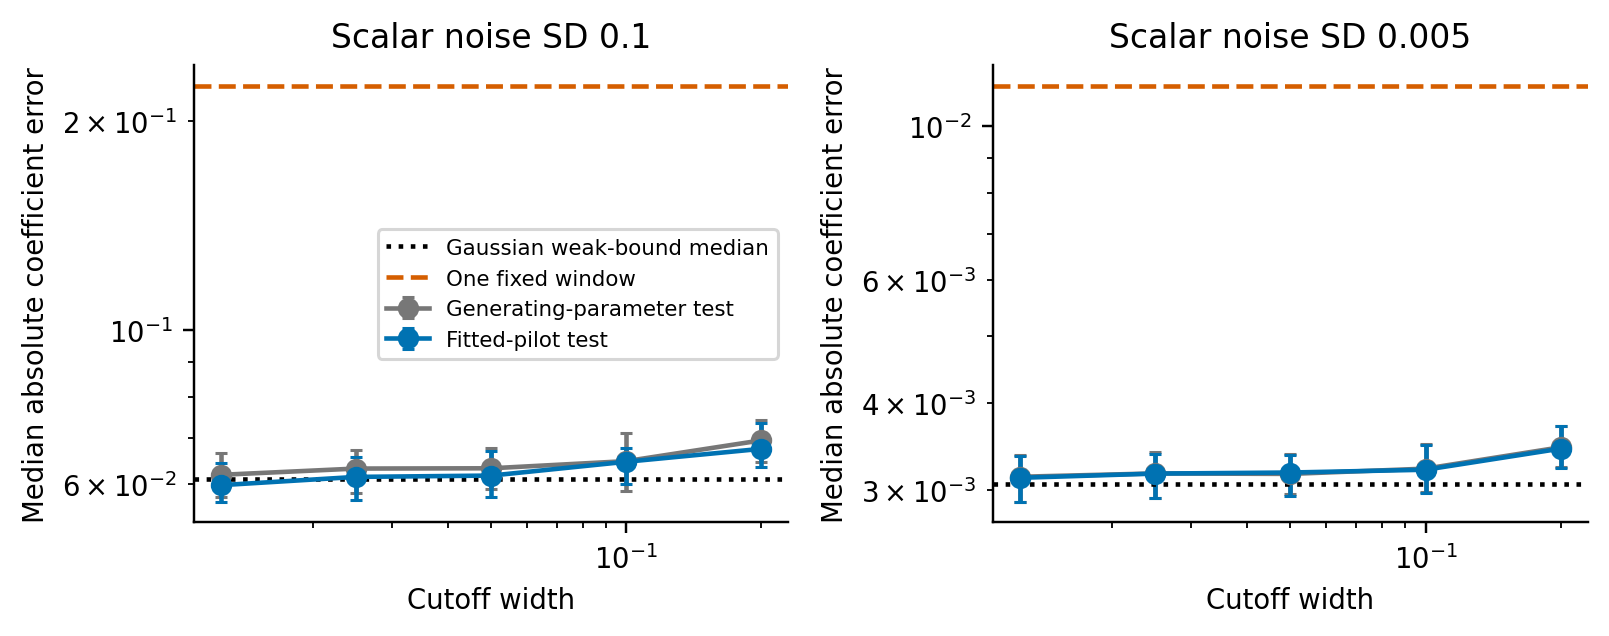
\includegraphics[keepaspectratio,alt={Figure 1. Scalar compact optimal tests at two noise amplitudes. Intervals resample independent paths; the dotted Gaussian median reference is derived from the sharp influence bound.}]{figures/publication/efficient_scalar.png}}
\caption{Scalar compact optimal tests at two noise amplitudes.
Intervals resample independent paths; the dotted Gaussian median
reference is derived from the sharp influence bound.}
\end{figure}

\subsubsection{7.2. Van der Pol: nested spans and temporal
weighting}\label{van-der-pol-nested-spans-and-temporal-weighting}

We estimate four independently free coefficients in \(x'=av\),
\(v'=bx+cv+dx^2v\), with truth \((1,-1,1,-1)\), initial state \((2,0)\),
\(T=20\), OU correlation time 0.3 and \(h=0.005\). Marginal coordinate
noise scales are fixed from the same clean \(h=0.01\) calibration as
S9.6. The relative error denominator is the Euclidean coefficient norm,
two. The continuous known-initial-state reference is 0.013093 at 5\%
noise; the sharp boundary-free relative RMSE reference is 0.016904. At
0.5\% noise these scale down by ten. Estimating a single tied oscillator
parameter would be a different information experiment (S9.7).

The nested families contain 30 full-width-three bumps; then 30 width-1.5
and 60 width-0.75 bumps; then 120 width-0.375 and 240 width-0.1875
bumps. A fixed \(H^1\) Gram transformation preserves their spans while
improving representation. Relative cutoff \(10^{-10}\) retains 30, 120
and 479 dimensions; the largest family has one linear dependence at this
numerical resolution. The smallest retained relative Gram eigenvalue in
that family is approximately \(2.1\times10^{-5}\). Covariance solves add
\(10^{-10}\) times the mean diagonal. This finite family is an
approximation experiment, not a proof of density for an infinite
sequence.

\begin{center}
\begin{minipage}{\linewidth}
Table 2. Oracle Gaussian influence RMSE under actual OU noise at 5\%.
Both methods use the same test span and clean design; they differ only
in the covariance used for GLS weights. Actual variance uses the OU
covariance for both.

\small\setlength{\tabcolsep}{3pt}
\begin{tabular}{@{}
  >{\raggedleft\arraybackslash}p{(\linewidth - 8\tabcolsep) * \real{0.2000}}
  >{\raggedleft\arraybackslash}p{(\linewidth - 8\tabcolsep) * \real{0.2000}}
  >{\raggedleft\arraybackslash}p{(\linewidth - 8\tabcolsep) * \real{0.2000}}
  >{\raggedleft\arraybackslash}p{(\linewidth - 8\tabcolsep) * \real{0.2000}}
  >{\raggedleft\arraybackslash}p{(\linewidth - 8\tabcolsep) * \real{0.2000}}@{}}
\toprule\noalign{}
\begin{minipage}[b]{\linewidth}\raggedleft
Prescribed windows
\end{minipage} & \begin{minipage}[b]{\linewidth}\raggedleft
Retained tests
\end{minipage} & \begin{minipage}[b]{\linewidth}\raggedleft
OU-weight RMSE
\end{minipage} & \begin{minipage}[b]{\linewidth}\raggedleft
iid-weight RMSE
\end{minipage} & \begin{minipage}[b]{\linewidth}\raggedleft
OU RMSE / class reference
\end{minipage} \\
\midrule\noalign{}
30 & 30 & 0.019605 & 0.020296 & 1.1597 \\
120 & 120 & 0.017043 & 0.017839 & 1.0082 \\
480 & 479 & 0.016938 & 0.017734 & 1.0020 \\
\bottomrule
\end{tabular}
\end{minipage}
\end{center}

The OU-weighted 480-window local reference is within 0.2\% in RMSE of
the class optimum; iid weighting retains a roughly 4.9\% gap. Optimal
weighting in the narrow 30-window span limits how much temporal
covariance can help. Expanding the span makes the distinction
observable. This is a verified prediction for the specified spans; it
does not imply that every iid-weighted dense family must have a positive
limiting gap. The independent exact-polynomial covariance fixture agrees
with Proposition 3 to relative error below \(10^{-14}\).

The largest clean discrete GLS coefficient error is 2.82e-07, below the
small-noise error scale. For the feasible test, 128 independent paths at
each amplitude are shared by both weights and all three families.
Hermite-corrected moments use known marginal variances. A 30-window OLS
pilot is clipped to a fixed physical parameter box and integrated from
the known initial state. Exact polynomial covariance is evaluated on
this fitted model trajectory, and coefficient-dependent weights are
updated for at most 100 iterations, with relative tolerance \(10^{-7}\).
The true trajectory is not supplied to this estimator. This is a
known-support WENDy-like component; the complete author WENDy benchmark
is documented separately in S6 and S9.6.

\begin{center}
\begin{minipage}{\linewidth}
Table 3. Feasible Van der Pol empirical relative RMSE and 95\% path
bootstrap intervals, with 128 paired paths per row. Bias and dispersion
refer to the OU-weighted coefficient errors; their squares sum to
empirical MSE. Final coefficient estimates are unbounded, so these
finite-cohort summaries do not assert finite unconditional moments.

\small\setlength{\tabcolsep}{3pt}
\begin{tabular}{@{}
  >{\raggedright\arraybackslash}p{(\linewidth - 10\tabcolsep) * \real{0.1304}}
  >{\raggedleft\arraybackslash}p{(\linewidth - 10\tabcolsep) * \real{0.1739}}
  >{\raggedleft\arraybackslash}p{(\linewidth - 10\tabcolsep) * \real{0.1739}}
  >{\raggedleft\arraybackslash}p{(\linewidth - 10\tabcolsep) * \real{0.1739}}
  >{\raggedleft\arraybackslash}p{(\linewidth - 10\tabcolsep) * \real{0.1739}}
  >{\raggedleft\arraybackslash}p{(\linewidth - 10\tabcolsep) * \real{0.1739}}@{}}
\toprule\noalign{}
\begin{minipage}[b]{\linewidth}\raggedright
Noise
\end{minipage} & \begin{minipage}[b]{\linewidth}\raggedleft
Windows
\end{minipage} & \begin{minipage}[b]{\linewidth}\raggedleft
OU RMSE (95\% interval)
\end{minipage} & \begin{minipage}[b]{\linewidth}\raggedleft
iid RMSE (95\% interval)
\end{minipage} & \begin{minipage}[b]{\linewidth}\raggedleft
OU bias
\end{minipage} & \begin{minipage}[b]{\linewidth}\raggedleft
OU dispersion
\end{minipage} \\
\midrule\noalign{}
0.5\% & 30 & 0.00200 {[}0.00181, 0.00220{]} & 0.00203 {[}0.00184,
0.00223{]} & 0.00027 & 0.00198 \\
0.5\% & 120 & 0.00173 {[}0.00156, 0.00190{]} & 0.00177 {[}0.00161,
0.00194{]} & 0.00010 & 0.00173 \\
0.5\% & 480 & 0.00174 {[}0.00157, 0.00190{]} & 0.00178 {[}0.00161,
0.00194{]} & 0.00011 & 0.00173 \\
5\% & 30 & 0.02711 {[}0.02437, 0.02993{]} & 0.02744 {[}0.02439,
0.03050{]} & 0.00900 & 0.02557 \\
5\% & 120 & 0.02545 {[}0.02277, 0.02810{]} & 0.02548 {[}0.02286,
0.02819{]} & 0.00770 & 0.02426 \\
5\% & 480 & 0.02558 {[}0.02288, 0.02833{]} & 0.02551 {[}0.02295,
0.02799{]} & 0.00814 & 0.02425 \\
\bottomrule
\end{tabular}
\end{minipage}
\end{center}

At 0.5\% noise, OU weighting with 480 windows gives empirical RMSE
0.001737, versus the sharp reference 0.001690. At 5\% noise it gives
0.025583, versus 0.016904; bias 0.008143 and dispersion 0.024253
identify finite-noise excess error. The stronger finite-noise assertion
that more windows alone would reach 0.016904 is therefore not supported
by this feasible implementation. The small-noise result and
deterministic geometry support the conditional efficiency mechanism,
while the moderate-noise result delimits it.

At 0.5\% noise, paired iid-minus-OU RMSE for 480 windows is 0.000038,
with 95\% interval {[}-0.000038, 0.000116{]}. At 5\% noise, paired
iid-minus-OU RMSE for 480 windows is -0.000075, with 95\% interval
{[}-0.001295, 0.001045{]}. Both paired intervals include zero: this
128-path experiment does not resolve a statistical advantage of OU over
iid weighting. Intervals are not adjusted for multiple comparisons. All
1536 final fits meet the stopping tolerance within 23 iterations, and no
pilot is clipped; the finite-noise gap persists after this convergence
control. Stopping counts are retained in S8; no path is excluded.

\begin{figure}[p]
\centering
\pandocbounded{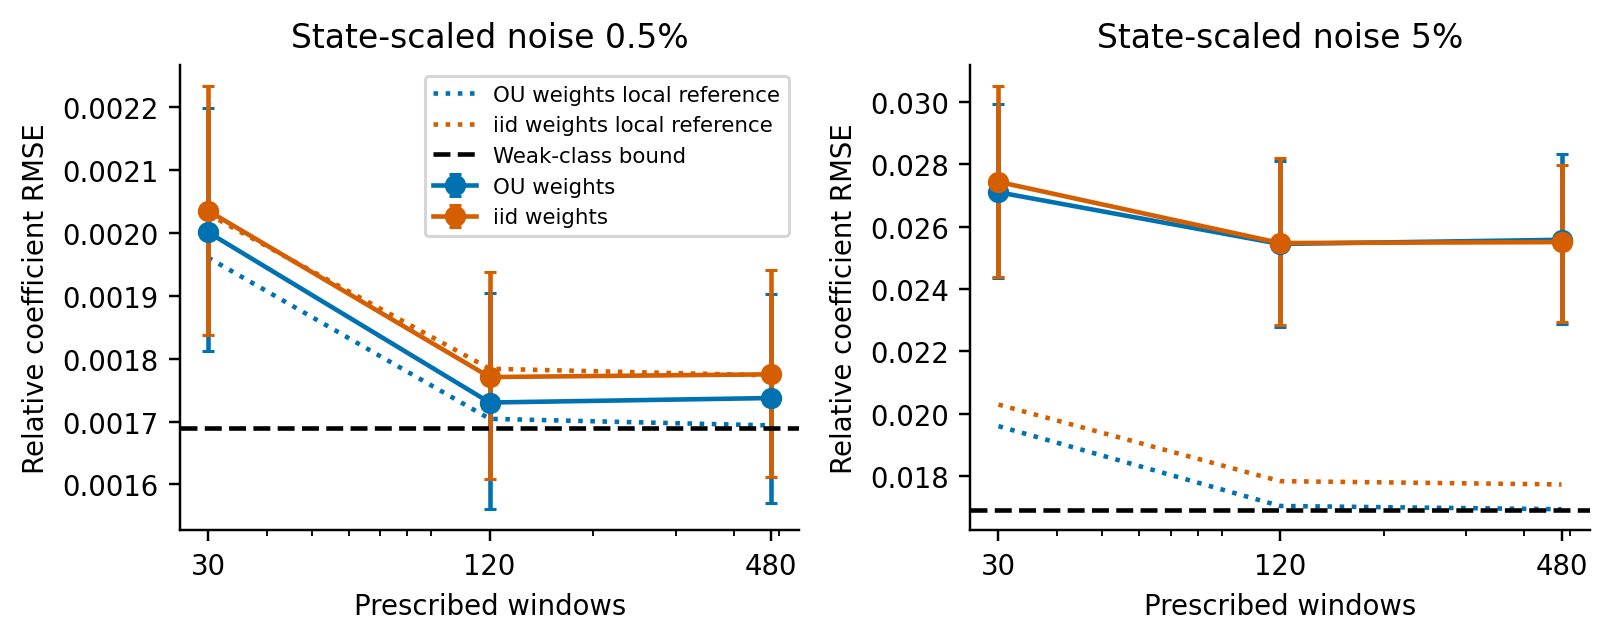
\includegraphics[keepaspectratio,alt={Figure 2. Feasible Van der Pol RMSE as the test span grows. Dotted curves show oracle local influences and the horizontal dashed line the class reference. Finite-noise estimation is distinguished from local Gaussian geometry.}]{figures/publication/efficient_vdp.png}}
\caption{Feasible Van der Pol RMSE as the test span grows.
Dotted curves show oracle local influences and the horizontal dashed
line the class reference. Finite-noise estimation is distinguished from
local Gaussian geometry.}
\end{figure}

\subsubsection{7.3. Supporting validation}\label{supporting-validation}

The supplement retains fixed-window sparse selection, coefficient
linearization checks, independent-record aggregation and 448 complete
adaptive author fits. These results provide context without constituting
a test of Corollary 1. In the separate 16-path 5\% OU comparison, full
WmSINDy has empirical RMSE 0.01926 and WENDy 0.02154, compared with the
weak reference 0.01690; their medians of approximately 0.015 do not
establish efficiency. Full coefficient and support distributions are
retained in S9.6--S9.7.

Stacking heterogeneous noisy regressions retains bias: the 16-record
empirical error decomposition is bias 0.03738, dispersion 0.00835 and
RMSE 0.03830. Approximately 95.3\% of empirical MSE is squared bias
(S9.9). In the coefficient covariance check all 2000 paths pass the
design guard, so it does not filter that finite sample. Its relative RMS
linearization discrepancy can exceed one because its denominator is the
RMS linear displacement (S3 and S9.3). These observations distinguish
covariance calculation, estimator bias and independent acquisition.

\subsection{8. Discussion and
limitations}\label{discussion-and-limitations}

The adjoint-range characterization turns the initial-sensitivity
constraint into an exact description of the closed influence class. Its
sharp optimum follows from classical Gaussian projection, and the OU
inverse covariance makes an optimal generalized test explicit. Endpoint
atoms explain why compact tests generally approach the optimum without
attaining it. The constructed scalar cutoff uses compact tests
throughout; this article does not test an estimator with additional
boundary terms.

Correct covariance weighting is optimal within a fixed span. Density in
the covariance norm is required to approach the class bound. A
well-conditioned representation changes computation, not the underlying
span. An explicit fundamental-matrix inverse may itself be
ill-conditioned for a contracting dynamical direction. The multiscale
calculation therefore uses a fixed, data-independent basis
transformation and reports retained dimensions and numerical relaxation.

Corollary 1 requires consistent pilots, correct covariance shape, a
regular local estimator, controlled quadrature and risk conditions. Its
limits are sequential. It does not prove a joint
window-growth/noise-decay limit, global convergence of covariance
iterations, efficiency after sparse support selection, or efficiency of
the released iid WENDy implementation under OU noise. A finite nested
family does not establish density of an infinite family. The iid
comparison tests a specified misspecification and does not establish a
universal limiting plateau.

Exact residual covariance and marginal Hermite correction address
distinct parts of the weak errors-in-variables problem. At finite noise,
random design and pilot errors can still produce bias and excess
dispersion. The numerical comparison therefore reports RMSE, bias,
dispersion, stopping diagnostics and uncertainty, rather than equating a
median error with a covariance bound. Supplementary complete-pipeline
results use a different 16-path protocol and are not pooled with the new
128-path experiment.

The analysis assumes fully observed deterministic ODEs and additive
stationary Gaussian measurement error with known positive covariance
common across parameters. Unknown covariance, partial observation and
process noise are outside the theorem proved here. The scope is an
information reference and its weak approximation, rather than a general
ranking of identification algorithms.

\subsection{Declaration of generative AI and AI-assisted
technologies}\label{declaration-of-generative-ai-and-ai-assisted-technologies}

OpenAI Codex assisted literature searches, mathematical drafting, source
development, experiment orchestration, numerical interpretation and
manuscript preparation. Numerical results are derived from archived
execution outputs, and figures are produced by plotting code. The tool
is not an author. The human authors must review and edit the manuscript
and accept responsibility for its content before submission; this
statement does not assert that their review has already occurred.

\subsection{Data availability}\label{data-availability}

Code, synthetic observations, numerical outputs and frozen execution
notebooks are available in the public
\href{https://github.com/malyshevdanil/wsindy-information-limits/tree/v1.1.0}{reproducibility
repository, version v1.1.0}. The repository includes protocol
configurations, source fingerprints, pinned author-code download
specifications, compatibility adapters, postprocessing scripts and
SHA256 manifests. Original author sources are downloaded from their
pinned repositories rather than redistributed. No external experimental
dataset is used. The tagged snapshot identifies the version supporting
this article; a DOI has not been assigned.

\subsection*{References}\label{references}
\addcontentsline{toc}{subsection}{References}

\protect\phantomsection\label{refs}
\begin{CSLReferences}{0}{0}
\bibitem[\citeproctext]{ref-brunton2016}
\CSLLeftMargin{{[}1{]} }%
\CSLRightInline{Brunton SL, Proctor JL, Kutz JN. Discovering governing
equations from data by sparse identification of nonlinear dynamical
systems. \emph{Proceedings of the National Academy of Sciences} 113
(2016) 3932--3937. \url{https://doi.org/10.1073/pnas.1517384113}.}

\bibitem[\citeproctext]{ref-schaeffer2017}
\CSLLeftMargin{{[}2{]} }%
\CSLRightInline{Schaeffer H, McCalla SG. Sparse model selection via
integral terms. \emph{Physical Review E} 96 (2017) 023302.
\url{https://doi.org/10.1103/PhysRevE.96.023302}.}

\bibitem[\citeproctext]{ref-messenger2021}
\CSLLeftMargin{{[}3{]} }%
\CSLRightInline{Messenger DA, Bortz DM. Weak {SINDy}: Galerkin-based
data-driven model selection. \emph{Multiscale Modeling and Simulation}
19 (2021) 1474--1497. \url{https://doi.org/10.1137/20M1343166}.}

\bibitem[\citeproctext]{ref-reinbold2020}
\CSLLeftMargin{{[}4{]} }%
\CSLRightInline{Reinbold PAK, Gurevich DR, Grigoriev RO. Using noisy or
incomplete data to discover models of spatiotemporal dynamics.
\emph{Physical Review E} 101 (2020) 010203.
\url{https://doi.org/10.1103/PhysRevE.101.010203}.}

\bibitem[\citeproctext]{ref-stein1999}
\CSLLeftMargin{{[}5{]} }%
\CSLRightInline{Stein ML. Interpolation of spatial data: Some theory for
kriging. Springer (1999)
\url{https://doi.org/10.1007/978-1-4612-1494-6}.}

\bibitem[\citeproctext]{ref-ying1991}
\CSLLeftMargin{{[}6{]} }%
\CSLRightInline{Ying Z. Asymptotic properties of a maximum likelihood
estimator with data from a gaussian process. \emph{Journal of
Multivariate Analysis} 36 (1991) 280--296.
\url{https://doi.org/10.1016/0047-259X(91)90062-7}.}

\bibitem[\citeproctext]{ref-zhang2004}
\CSLLeftMargin{{[}7{]} }%
\CSLRightInline{Zhang H. Inconsistent estimation and asymptotically
equal interpolations in model-based geostatistics. \emph{Journal of the
American Statistical Association} 99 (2004) 250--261.
\url{https://doi.org/10.1198/016214504000000241}.}

\bibitem[\citeproctext]{ref-dette2016}
\CSLLeftMargin{{[}8{]} }%
\CSLRightInline{Dette H, Pepelyshev A, Zhigljavsky A. Optimal designs in
regression with correlated errors. \emph{The Annals of Statistics} 44
(2016) 113--152. \url{https://doi.org/10.1214/15-AOS1361}.}

\bibitem[\citeproctext]{ref-messenger2025}
\CSLLeftMargin{{[}9{]} }%
\CSLRightInline{Messenger DA, Bortz DM. Asymptotic consistency of the
{WSINDy} algorithm in the limit of continuum data. \emph{IMA Journal of
Numerical Analysis} 45 (2025) 3264--3312.
\url{https://doi.org/10.1093/imanum/drae086}.}

\bibitem[\citeproctext]{ref-isserlis1918}
\CSLLeftMargin{{[}10{]} }%
\CSLRightInline{Isserlis L. On a formula for the product-moment
coefficient of any order of a normal frequency distribution in any
number of variables. \emph{Biometrika} 12 (1918) 134--139.
\url{https://doi.org/10.1093/biomet/12.1-2.134}.}

\bibitem[\citeproctext]{ref-bortz2023}
\CSLLeftMargin{{[}11{]} }%
\CSLRightInline{Bortz DM, Messenger DA, Dukic V. Direct estimation of
parameters in {ODE} models using {WENDy}: Weak-form estimation of
nonlinear dynamics. \emph{Bulletin of Mathematical Biology} 85 (2023)
110. \url{https://doi.org/10.1007/s11538-023-01208-6}.}

\bibitem[\citeproctext]{ref-fuller1987}
\CSLLeftMargin{{[}12{]} }%
\CSLRightInline{Fuller WA. Measurement error models. Wiley (1987)
\url{https://doi.org/10.1002/9780470316665}.}

\bibitem[\citeproctext]{ref-stefanski1989}
\CSLLeftMargin{{[}13{]} }%
\CSLRightInline{Stefanski LA. Unbiased estimation of a nonlinear
function of a normal mean with application to measurement error models.
\emph{Communications in Statistics - Theory and Methods} 18 (1989)
4335--4358. \url{https://doi.org/10.1080/03610928908830159}.}

\bibitem[\citeproctext]{ref-ramsay2007}
\CSLLeftMargin{{[}14{]} }%
\CSLRightInline{Ramsay JO, Hooker G, Campbell D, Cao J. Parameter
estimation for differential equations: A generalized smoothing approach.
\emph{Journal of the Royal Statistical Society: Series B} 69 (2007)
741--796. \url{https://doi.org/10.1111/j.1467-9868.2007.00610.x}.}

\bibitem[\citeproctext]{ref-lopez2026}
\CSLLeftMargin{{[}15{]} }%
\CSLRightInline{López C, Naranjo Á, Salazar D, Moore KJ. Weak-form
modified sparse identification of nonlinear dynamics. \emph{Journal of
Computational Physics} 544 (2026) 114410.
\url{https://doi.org/10.1016/j.jcp.2025.114410}.}

\bibitem[\citeproctext]{ref-fasel2022}
\CSLLeftMargin{{[}16{]} }%
\CSLRightInline{Fasel U, Kutz JN, Brunton BW, Brunton SL.
Ensemble-{SINDy}: Robust sparse model discovery in the low-data,
high-noise limit, with active learning and control. \emph{Proceedings of
the Royal Society A} 478 (2022) 20210904.
\url{https://doi.org/10.1098/rspa.2021.0904}.}

\bibitem[\citeproctext]{ref-uhlenbeck1930}
\CSLLeftMargin{{[}17{]} }%
\CSLRightInline{Uhlenbeck GE, Ornstein LS. On the theory of the brownian
motion. \emph{Physical Review} 36 (1930) 823--841.
\url{https://doi.org/10.1103/PhysRev.36.823}.}

\bibitem[\citeproctext]{ref-cameron1944}
\CSLLeftMargin{{[}18{]} }%
\CSLRightInline{Cameron RH, Martin WT. Transformations of weiner
integrals under translations. \emph{Annals of Mathematics} 45 (1944)
386--396. \url{https://doi.org/10.2307/1969276}.}

\bibitem[\citeproctext]{ref-feldman1958}
\CSLLeftMargin{{[}19{]} }%
\CSLRightInline{Feldman J. Equivalence and perpendicularity of gaussian
processes. \emph{Pacific Journal of Mathematics} 8 (1958) 699--708.
\url{https://doi.org/10.2140/pjm.1958.8.699}.}

\end{CSLReferences}

\end{document}
